\documentclass[man]{apa6}
\usepackage{lmodern}
\usepackage{amssymb,amsmath}
\usepackage{ifxetex,ifluatex}
\usepackage{fixltx2e} % provides \textsubscript
\ifnum 0\ifxetex 1\fi\ifluatex 1\fi=0 % if pdftex
  \usepackage[T1]{fontenc}
  \usepackage[utf8]{inputenc}
\else % if luatex or xelatex
  \ifxetex
    \usepackage{mathspec}
  \else
    \usepackage{fontspec}
  \fi
  \defaultfontfeatures{Ligatures=TeX,Scale=MatchLowercase}
\fi
% use upquote if available, for straight quotes in verbatim environments
\IfFileExists{upquote.sty}{\usepackage{upquote}}{}
% use microtype if available
\IfFileExists{microtype.sty}{%
\usepackage{microtype}
\UseMicrotypeSet[protrusion]{basicmath} % disable protrusion for tt fonts
}{}
\usepackage{hyperref}
\hypersetup{unicode=true,
            pdftitle={Reproducing the analysis of Rosenbaum, Mama, \& Algom (2017)},
            pdfauthor={Matthew Crump},
            pdfkeywords={Stroop, Reproducibilty},
            pdfborder={0 0 0},
            breaklinks=true}
\urlstyle{same}  % don't use monospace font for urls
\usepackage{graphicx,grffile}
\makeatletter
\def\maxwidth{\ifdim\Gin@nat@width>\linewidth\linewidth\else\Gin@nat@width\fi}
\def\maxheight{\ifdim\Gin@nat@height>\textheight\textheight\else\Gin@nat@height\fi}
\makeatother
% Scale images if necessary, so that they will not overflow the page
% margins by default, and it is still possible to overwrite the defaults
% using explicit options in \includegraphics[width, height, ...]{}
\setkeys{Gin}{width=\maxwidth,height=\maxheight,keepaspectratio}
\IfFileExists{parskip.sty}{%
\usepackage{parskip}
}{% else
\setlength{\parindent}{0pt}
\setlength{\parskip}{6pt plus 2pt minus 1pt}
}
\setlength{\emergencystretch}{3em}  % prevent overfull lines
\providecommand{\tightlist}{%
  \setlength{\itemsep}{0pt}\setlength{\parskip}{0pt}}
\setcounter{secnumdepth}{0}
% Redefines (sub)paragraphs to behave more like sections
\ifx\paragraph\undefined\else
\let\oldparagraph\paragraph
\renewcommand{\paragraph}[1]{\oldparagraph{#1}\mbox{}}
\fi
\ifx\subparagraph\undefined\else
\let\oldsubparagraph\subparagraph
\renewcommand{\subparagraph}[1]{\oldsubparagraph{#1}\mbox{}}
\fi

%%% Use protect on footnotes to avoid problems with footnotes in titles
\let\rmarkdownfootnote\footnote%
\def\footnote{\protect\rmarkdownfootnote}


  \title{Reproducing the analysis of Rosenbaum, Mama, \& Algom (2017)}
    \author{Matthew Crump\textsuperscript{1}}
    \date{}
  
\shorttitle{Stroop Analysis}
\affiliation{
\vspace{0.5cm}
\textsuperscript{1} Brooklyn College of the City University of New York}
\keywords{Stroop, Reproducibilty\newline\indent Word count: X}
\usepackage{csquotes}
\usepackage{upgreek}
\captionsetup{font=singlespacing,justification=justified}

\usepackage{longtable}
\usepackage{lscape}
\usepackage{multirow}
\usepackage{tabularx}
\usepackage[flushleft]{threeparttable}
\usepackage{threeparttablex}

\newenvironment{lltable}{\begin{landscape}\begin{center}\begin{ThreePartTable}}{\end{ThreePartTable}\end{center}\end{landscape}}

\makeatletter
\newcommand\LastLTentrywidth{1em}
\newlength\longtablewidth
\setlength{\longtablewidth}{1in}
\newcommand{\getlongtablewidth}{\begingroup \ifcsname LT@\roman{LT@tables}\endcsname \global\longtablewidth=0pt \renewcommand{\LT@entry}[2]{\global\advance\longtablewidth by ##2\relax\gdef\LastLTentrywidth{##2}}\@nameuse{LT@\roman{LT@tables}} \fi \endgroup}


\DeclareDelayedFloatFlavor{ThreePartTable}{table}
\DeclareDelayedFloatFlavor{lltable}{table}
\DeclareDelayedFloatFlavor*{longtable}{table}
\makeatletter
\renewcommand{\efloat@iwrite}[1]{\immediate\expandafter\protected@write\csname efloat@post#1\endcsname{}}
\makeatother

\authornote{Add complete departmental affiliations for each author here. Each new line herein must be indented, like this line.

Correspondence concerning this article should be addressed to Matthew Crump, 2900 Bedford Ave. E-mail: \href{mailto:mcrump@brooklyn.cuny.edu}{\nolinkurl{mcrump@brooklyn.cuny.edu}}}

\abstract{
A reproduction of the analysis for Experiment 3 from Rosenbaum, Mama, and Algom (2017).


}

\begin{document}
\maketitle

This is an example of creating an APA manuscript using papaja, and also an example for part 2 of the midterm assignment. Another sentence.

This report re-produces the analysis of Experiment 3 reported in Rosenbaum, Mama, and Algom (2017). The data were downloaded from \url{https://osf.io/b7x8q/}

Rosenbaum et al. (2017) had participants perform a Stroop task in one of two posture conditions. Participants either sat and performed the Stroop task, or stood and performed the Stroop task. The question was whether the size of the Stroop effect would change as a function of posture. The Stroop effect is measured as a difference between reaction times on congruent vs.~incongruent trials.The experiment involved a 2 (Posture: sitting vs standing) x 2 (congruency: congruent vs.~incongruent) repeated measures design.

\hypertarget{methods}{%
\section{Methods}\label{methods}}

\hypertarget{participants}{%
\subsection{Participants}\label{participants}}

There were 50 participants

\hypertarget{material}{%
\subsection{Material}\label{material}}

The details of the Stroop experiment are report in Rosenbaum et al. (2017)

\hypertarget{procedure}{%
\subsection{Procedure}\label{procedure}}

In each posture condition, participants completed 72 Stroop trials, half congruent and half incongruent.

\hypertarget{results}{%
\section{Results}\label{results}}

Mean reaction times for each subject in each condition to a 2 (Congruency: congruent vs.~incongruent) x 2 (Posture: Standing vs.~Sitting) were submitted to a repeated measures ANOVA. Mean RTs in each condition are displayed in Table 1, and in Figure 1. The full ANOVA table is reported in Table 2.

\begin{table}

\caption{\label{tab:unnamed-chunk-2}Mean Reaction Times and Standard Errors of the Mean for Experiment 3}
\centering
\begin{tabular}[t]{lrrrr}
\toprule
\multicolumn{1}{c}{ } & \multicolumn{2}{c}{Congruent} & \multicolumn{2}{c}{Incongruent} \\
\cmidrule(l{2pt}r{2pt}){2-3} \cmidrule(l{2pt}r{2pt}){4-5}
Posture & RT & SEM & RT & SEM\\
\midrule
Sit & 822 & 17 & 941 & 18\\
Stand & 808 & 15 & 904 & 15\\
\bottomrule
\end{tabular}
\end{table}

\begin{figure}
\centering
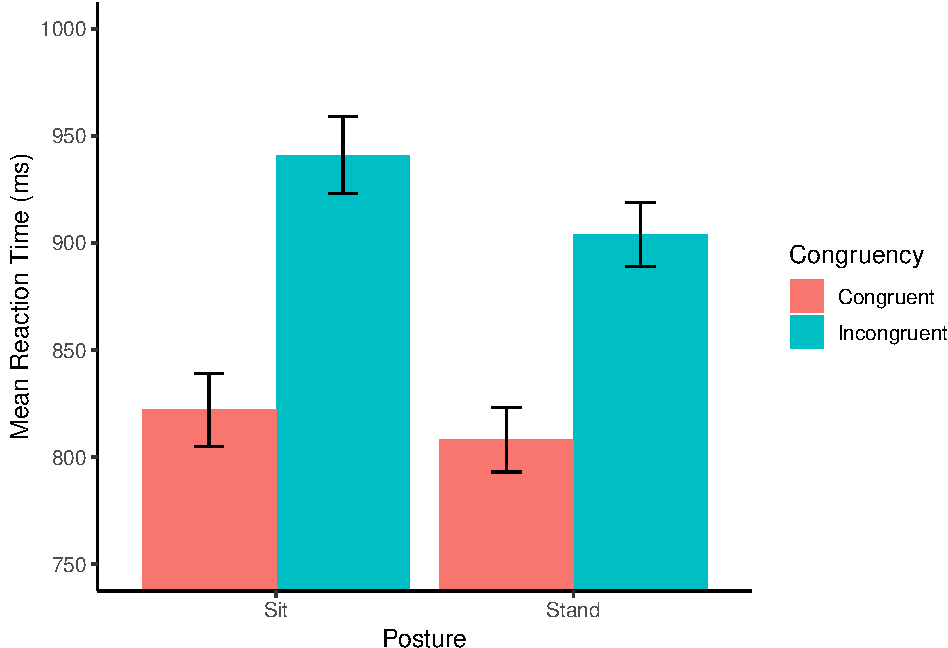
\includegraphics{APAreport_files/figure-latex/stroopfig-1.pdf}
\caption{\label{fig:stroopfig}Mean reaction times wth standard error bars as a function of Posture and Congruency for Experiment 3}
\end{figure}

\begin{table}[tbp]
\begin{center}
\begin{threeparttable}
\caption{\label{tab:aovtable}ANOVA table for Experiment 3}
\begin{tabular}{lllllll}
\toprule
Effect & \multicolumn{1}{c}{$F$} & \multicolumn{1}{c}{$\mathit{df}_1$} & \multicolumn{1}{c}{$\mathit{df}_2$} & \multicolumn{1}{c}{$\mathit{MSE}$} & \multicolumn{1}{c}{$p$} & \multicolumn{1}{c}{$\hat{\eta}^2_G$}\\
\midrule
Posture & 7.33 & 1 & 49 & 4,407.09 & .009 & .012\\
Congruency & 342.45 & 1 & 49 & 1,684.39 & < .001 & .182\\
Posture $\times$ Congruency & 8.96 & 1 & 49 & 731.82 & .004 & .003\\
\bottomrule
\end{tabular}
\end{threeparttable}
\end{center}
\end{table}

Below are examples of writing the results using two methods. The first method is to report all of the values by hand. The second method is to embed the results of R variables into the reporting using papaja. Both results sections appear similar in the .pdf, so look at the .rmd file for this example to see how to use papaja.

\hypertarget{by-hand-reporting}{%
\subsection{By hand reporting}\label{by-hand-reporting}}

There was a main effect of Congruency, F (1, 49) = 342.45, MSE = 1684.39, p \textless{} 0.001. Mean reaction times were slower for incongruent (922 ms) than congruent groups (815 ms).

There main effect of Posture was significant, F (1, 49) = 7.33, MSE = 4407.09, p =.009. Mean reaction times were slower for sitting (881 ms) than standing groups (855 ms).

The two-way interaction between Congruency and Posture was significant, F (1, 49) = 8.96, MSE = 731.82, p \textless{} 0.004. The Stroop effect was 23 ms smaller in the standing than sitting conditions.

\hypertarget{papaja-reporting}{%
\subsection{papaja reporting}\label{papaja-reporting}}

There was a main effect of Congruency, \(F(1, 49) = 342.45\), \(\mathit{MSE} = 1,684.39\), \(p < .001\), \(\hat{\eta}^2_G = .182\). Mean reaction times were slower for incongruent (922 ms) than congruent groups (815 ms).

There main effect of Posture was significant, \(F(1, 49) = 7.33\), \(\mathit{MSE} = 4,407.09\), \(p = .009\), \(\hat{\eta}^2_G = .012\). Mean reaction times were slower for sitting (881 ms) than standing groups (855 ms).

The two-way interaction between Congruency and Posture was significant, \(F(1, 49) = 8.96\), \(\mathit{MSE} = 731.82\), \(p = .004\), \(\hat{\eta}^2_G = .003\). The Stroop effect was 23 ms smaller in the standing than sitting conditions.

\hypertarget{discussion}{%
\section{Discussion}\label{discussion}}

The re-analysis successfully reproduced the analysis reported by Rosenbaum et al. (2017). In the following section, I show an example of completing a simulation based power analysis for this design.

\hypertarget{simulation-based-power-analysis}{%
\subsection{Simulation-based power analysis}\label{simulation-based-power-analysis}}

The design was a 2x2 repeated measures design with 50 subjects. This design leads to three different effects, the main effect of congruency, the main effect of posture, and the posture by congruency interaction. A power analysis could be applied to any of these effects. I will show examples for the main effect of congruency first, and then for the interaction.

Several features of the design can go into the power analysis, the major ones being the number of subjects, the effect-size, and assumptions about the distributions underlying the sample data. Power is the probability that the design will reject the null-hypothesis, when the null-hypothesis is false and there is a true difference. Power depends on the size of the true difference. The same design will have greater power to detect a large versus small difference. Commonly, the assumed true difference is defined in terms of Cohen's D, a mean difference in terms of standard deviation units.

We will first estimate the overall mean reaction time, and the standard deviation of the mean reaction from the data. The overall mean was 868.65, and the overall standard deviation was 107.16.

To conduct the simulation we generate data for each subject using the rnorm function. Each subject contributed had two mean RTs in the congruent condition (sitting and standing), and two mean RTs in the incongruent condition (sitting and standing). There were 50 subjects, for the congruent condition we sample 2 scores for each subject from the above normal distribution (100 total scores), and 2 scores for each subject from the above normal distribution for the incongruent condition (100 total scores). To model the Stroop effect, we systemically increase the mean in the incongruent condition by a proportion of the standard deviation. We use effect-sizes of .05, .1, .2, .4, .5, and .8; which range from small to large. For each effect-size, we run 100 simulated experiments, and save p-value for the main effect of congruency for each simulated experiment. Then, for each effect-size, we find the proportion of experiments that resulted in p\textless{}.05. The proportion of experiments that reject the null is the power of the design to detect an effect of each size. The simulation below finds that this design had power of .8, to detect an effect of d=.4. It had power of .99 to detect effects of d=.8 or larger. The full power-curve for this design is displayed in Figure 2.

\begin{figure}
\centering
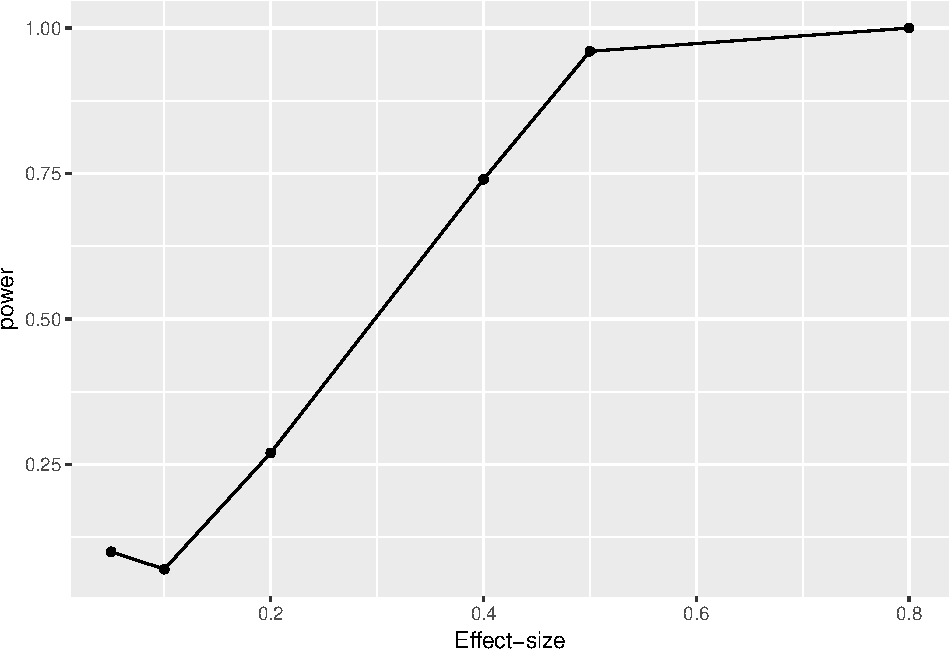
\includegraphics{APAreport_files/figure-latex/powerfig-1.pdf}
\caption{\label{fig:powerfig}Simulation-based power curve for this design}
\end{figure}

\newpage

\hypertarget{references}{%
\section{References}\label{references}}

\begingroup
\setlength{\parindent}{-0.5in}
\setlength{\leftskip}{0.5in}

\hypertarget{refs}{}
\leavevmode\hypertarget{ref-rosenbaum2017stand}{}%
Rosenbaum, D., Mama, Y., \& Algom, D. (2017). Stand by your stroop: Standing up enhances selective attention and cognitive control. \emph{Psychological Science}, \emph{28}(12), 1864--1867.

\endgroup


\end{document}
